\begin{flushleft}
	{\color{blue!50!green}\fbox{\fontfamily{qag}\bfseries\selectfont PHẦN I. Câu trắc nghiệm nhiều phương án lựa chọn}}
	\textit{\small (Thí sinh trả lời từ câu 1 đến câu 12. Mỗi câu hỏi thí sinh chỉ chọn một phương án.)}
\end{flushleft}
\setcounter{ex}{0}
\setcounter{bt}{0}

% Câu 1
\begin{ex}
	\macau{ID: TOAN12-BT3-0104-C01}Cho hàm số $y = f(x)$ có đạo hàm $f'(x) = 3(x - 1)(x - 3)$ với mọi $x \in \mathbb{R}$. Khoảng nghịch biến của hàm số là
	\choice
	{$(-\infty; 1)$}
	{$(3; +\infty)$}
	{$(-\infty; 3)$}
	{\True $(1; 3)$}
	\loigiai{
		Ta có $f'(x) < 0 \iff 3(x - 1)(x - 3) < 0 \iff 1 < x < 3$.\\
		Vậy hàm số nghịch biến trên khoảng $(1; 3)$.
	}
\end{ex}

% Câu 2
\begin{ex}
	\macau{ID: TOAN12-BT3-0104-C02}Cho hàm số $y = f(x)$ có bảng biến thiên như dưới đây:
	\begin{center}
	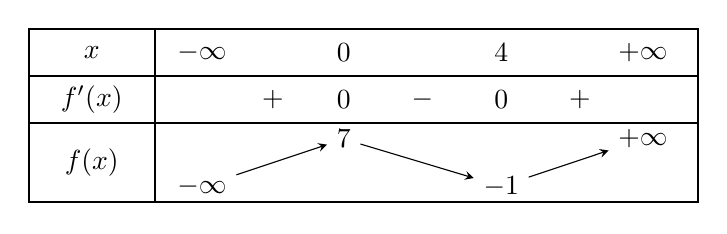
\begin{tikzpicture}[>=stealth,scale=1]
	  \draw[thick] (0,0) rectangle (8.5,-2.2);
	  \draw[thick] (0,-0.6) -- (8.5,-0.6);
	  \draw[thick] (0,-1.2) -- (8.5,-1.2);
	  \draw[thick] (1.6,0) -- (1.6,-2.2);
	  \node at (0.8,-0.3) {$x$};
	  \node at (0.8,-0.9) {$f'(x)$};
	  \node at (0.8,-1.7) {$f(x)$};
	  \node at (2.2,-0.3) {$-\infty$};
	  \node at (4.0,-0.3) {$0$};
	  \node at (6.0,-0.3) {$4$};
	  \node at (7.8,-0.3) {$+\infty$};
	  \node at (3.1,-0.9) {$+$};
	  \node at (4.0,-0.9) {$0$};
	  \node at (5.0,-0.9) {$-$};
	  \node at (6.0,-0.9) {$0$};
	  \node at (7.0,-0.9) {$+$};
	  \node (p1) at (2.2,-2.0) {$-\infty$};
	  \node (p2) at (4.0,-1.4) {$7$};
	  \node (p3) at (6.0,-2.0) {$-1$};
	  \node (p4) at (7.8,-1.4) {$+\infty$};
	  \draw[->] (p1) -- (p2);
	  \draw[->] (p2) -- (p3);
	  \draw[->] (p3) -- (p4);
	\end{tikzpicture}
	\end{center}
	Giá trị cực đại của hàm số là
	\choice
	{$0$}
	{\True $7$}
	{$4$}
	{$-1$}
	\loigiai{
		Từ bảng biến thiên, khi qua $x = 0$, đạo hàm $f'(x)$ đổi dấu từ dương sang âm nên hàm số đạt cực đại tại $x = 0$ và giá trị cực đại là $y_{\text{CĐ}} = 7$.
	}
\end{ex}

% Câu 3
\begin{ex}
	\macau{ID: TOAN12-BT3-0104-C03}Cho hàm số $y = \dfrac{3x - 2}{x + 4}$. Phương trình tiệm cận đứng là
	\choice
	{\True $x = -4$}
	{$x = 4$}
	{$y = 3$}
	{$y = -4$}
	\loigiai{
		Ta có $\lim\limits_{x \to (-4)^+} \dfrac{3x - 2}{x + 4} = -\infty$ và $\lim\limits_{x \to (-4)^-} \dfrac{3x - 2}{x + 4} = +\infty$. Vậy đường tiệm cận đứng của đồ thị hàm số là $x = -4$.
	}
\end{ex}

\newpage
% Câu 4
\begin{ex}
	\macau{ID: TOAN12-BT3-0104-C04}Cho hàm số $y = \dfrac{-2x + 5}{x - 1}$. Phương trình tiệm cận ngang là
	\choice
	{$y = 2$}
	{$x = 1$}
	{\True $y = -2$}
	{$y = 5$}
	\loigiai{
		Ta có $\lim\limits_{x \to \pm\infty} \dfrac{-2x + 5}{x - 1} = -2$. Do đó đường tiệm cận ngang của đồ thị hàm số có phương trình là $y = -2$.
	}
\end{ex}

% Câu 5
\begin{ex}
	\macau{ID: TOAN12-BT3-0104-C05}Cho hàm số $y = x - 1 + \dfrac{2}{x - 2}$. Phương trình đường tiệm cận xiên của đồ thị hàm số là
	\choice
	{$y = x + 1$}
	{\True $y = x - 1$}
	{$y = -x + 1$}
	{$x = 2$}
	\loigiai{
		Ta có $\lim\limits_{x \to \pm\infty} [y - (x - 1)] = \lim\limits_{x \to \pm\infty} \dfrac{2}{x - 2} = 0$. Vậy đường thẳng $y = x - 1$ là đường tiệm cận xiên của đồ thị hàm số.
	}
\end{ex}

% Câu 6
\begin{ex}
	\macau{ID: TOAN12-BT3-0104-C06}Đồ thị hàm số $y = -3 + \dfrac{5}{x + 2}$ có tâm đối xứng là
	\choice
	{$I(2; -3)$}
	{$I(-3; 2)$}
	{$I(-2; 3)$}
	{\True $I(-2; -3)$}
	\loigiai{
		Đồ thị hàm số có tiệm cận đứng $x = -2$ và tiệm cận ngang $y = -3$. Giao điểm hai đường tiệm cận là tâm đối xứng của đồ thị: $I(-2; -3)$.
	}
\end{ex}

% Câu 7
\begin{ex}
	\macau{ID: TOAN12-BT3-0104-C07}Cho hàm số $y = f(x)$ có đạo hàm $f'(x) = (x + 1)^2(x - 2)(x - 5)$ với mọi $x \in \mathbb{R}$. Số điểm cực trị của hàm số là
	\choice
	{$1$}
	{$3$}
	{$4$}
	{\True $2$}
	\loigiai{
		Phương trình $f'(x) = 0 \iff x = -1$ (nghiệm bội $2$) hoặc $x = 2$ (nghiệm đơn) hoặc $x = 5$ (nghiệm đơn). Đạo hàm chỉ đổi dấu khi qua hai nghiệm đơn $x = 2$ và $x = 5$. Vậy hàm số có đúng $2$ điểm cực trị.
	}
\end{ex}

% Câu 8
\begin{ex}
	\macau{ID: TOAN12-BT3-0104-C08}Cho hàm số $y = x + 1 + \dfrac{3}{x - 1}$. Giao điểm hai đường tiệm cận của đồ thị hàm số là
	\choice
	{$I(1; 1)$}
	{\True $I(1; 2)$}
	{$I(-1; 0)$}
	{$I(2; 1)$}
	\loigiai{
		Đồ thị hàm số có đường tiệm cận đứng $x = 1$ và đường tiệm cận xiên $y = x + 1$. Tọa độ giao điểm hai đường tiệm cận là $I(1; 2)$ vì $y(1) = 1 + 1 = 2$.
	}
\end{ex}

\newpage
% Câu 9
\begin{ex}
	\immini{\macau{ID: TOAN12-BT3-0104-C09}
		Cho hàm số phân thức $y = \dfrac{ax + b}{cx + d}$ ($ac \ne 0$, $ad - bc \ne 0$) có đồ thị như hình bên. Hàm số nào dưới đây có đồ thị như hình đã cho?
		\choice
		{\True $y = 1 + \dfrac{2}{x + 1}$}
		{$y = 1 - \dfrac{2}{x + 1}$}
		{$y = 1 + \dfrac{2}{x - 1}$}
		{$y = -1 + \dfrac{2}{x + 1}$}
	}{
		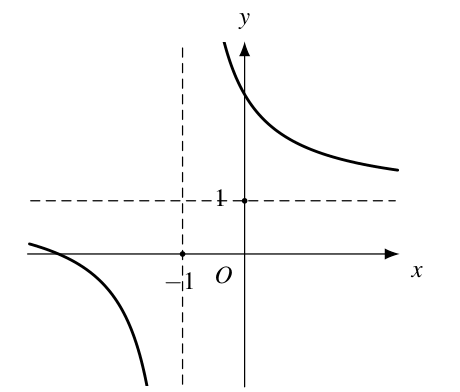
\includegraphics[width=4.0cm]{c9_hinh.png}
	}
	\loigiai{
		Từ đồ thị ta thấy:
		\begin{itemize}
			\item Tiệm cận đứng $x = -1$ (loại phương án C).
			\item Tiệm cận ngang $y = 1$ (loại phương án D).
			\item Tại $x = 0$, đồ thị cắt trục tung tại điểm có tung độ $y > 1$. Với hàm số $y = 1 + \dfrac{2}{x + 1}$, khi $x = 0 \implies y = 3 > 1$ (thỏa mãn).
		\end{itemize}
		Vậy hàm số có đồ thị như hình vẽ là $y = 1 + \dfrac{2}{x + 1}$.
	}
\end{ex}

% Câu 10
\begin{ex}
	\macau{ID: TOAN12-BT3-0104-C10}Cho hàm số $y = f(x)$ xác định trên $\mathbb{R} \setminus \{0\}$ và có đạo hàm $f'(x) = \dfrac{x^2 - 1}{x^2}$. Số điểm cực trị của hàm số là
	\choice
	{$0$}
	{$1$}
	{\True $2$}
	{$3$}
	\loigiai{
		Tập xác định $D = \mathbb{R} \setminus \{0\}$. Ta có $f'(x) = 0 \iff x^2 - 1 = 0 \iff x = \pm 1$. Vì qua $x = -1$ và $x = 1$, $f'(x)$ đều đổi dấu và các điểm này đều thuộc tập xác định nên hàm số có đúng $2$ điểm cực trị.
	}
\end{ex}

% Câu 11
\begin{ex}
	\macau{ID: TOAN12-BT3-0104-C11}Cho hàm số $y = f(x) = x^3 - 12x + 1$. Khẳng định nào sau đây đúng?
	\choice
	{\True Hàm số đạt cực trị tại $x = -2$ và $x = 2$}
	{Hàm số không có cực trị}
	{Hàm số có một điểm cực trị}
	{Tâm đối xứng của đồ thị là $I(1; 0)$}
	\loigiai{
		Ta có $f'(x) = 3x^2 - 12 = 3(x^2 - 4) = 0 \iff x = \pm 2$. Đạo hàm đổi dấu qua cả hai điểm này nên hàm số đạt cực trị tại $x = -2$ và $x = 2$. Tâm đối xứng của đồ thị là điểm uốn $I(0; 1)$.
	}
\end{ex}

% Câu 12
\begin{ex}
	\macau{ID: TOAN12-BT3-0104-C12}Cho hàm số bậc ba $y = f(x)$ có bảng biến thiên như dưới đây:
	\begin{center}
	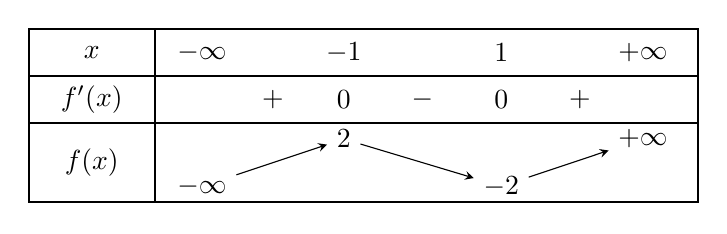
\begin{tikzpicture}[>=stealth,scale=1]
	  \draw[thick] (0,0) rectangle (8.5,-2.2);
	  \draw[thick] (0,-0.6) -- (8.5,-0.6);
	  \draw[thick] (0,-1.2) -- (8.5,-1.2);
	  \draw[thick] (1.6,0) -- (1.6,-2.2);
	  \node at (0.8,-0.3) {$x$};
	  \node at (0.8,-0.9) {$f'(x)$};
	  \node at (0.8,-1.7) {$f(x)$};
	  \node at (2.2,-0.3) {$-\infty$};
	  \node at (4.0,-0.3) {$-1$};
	  \node at (6.0,-0.3) {$1$};
	  \node at (7.8,-0.3) {$+\infty$};
	  \node at (3.1,-0.9) {$+$};
	  \node at (4.0,-0.9) {$0$};
	  \node at (5.0,-0.9) {$-$};
	  \node at (6.0,-0.9) {$0$};
	  \node at (7.0,-0.9) {$+$};
	  \node (p1) at (2.2,-2.0) {$-\infty$};
	  \node (p2) at (4.0,-1.4) {$2$};
	  \node (p3) at (6.0,-2.0) {$-2$};
	  \node (p4) at (7.8,-1.4) {$+\infty$};
	  \draw[->] (p1) -- (p2);
	  \draw[->] (p2) -- (p3);
	  \draw[->] (p3) -- (p4);
	\end{tikzpicture}
	\end{center}
	Hàm số nào dưới đây có bảng biến thiên đã cho?
	\choice
	{$y = -x^3 + 3x$}
	{$y = x^3 + 3x$}
	{\True $y = x^3 - 3x$}
	{$y = x^3 - 3x + 1$}
	\loigiai{
		Từ bảng biến thiên, khi $x \to +\infty$ thì $y \to +\infty$ nên hệ số bậc ba $a > 0$ (loại A). Hàm số có cực đại $y_{\text{CĐ}} = 2$ tại $x = -1$ và cực tiểu $y_{\text{CT}} = -2$ tại $x = 1$. Thử hàm số $y = x^3 - 3x$ ta có $y' = 3x^2 - 3 = 0 \iff x = \pm 1$; $y(-1) = 2$, $y(1) = -2$, hoàn toàn khớp với bảng biến thiên.
	}
\end{ex}

\newpage
\begin{flushleft}
	{\color{blue!50!green}\fbox{\fontfamily{qag}\bfseries\selectfont PHẦN II. Câu trắc nghiệm đúng sai}}
	\textit{\small (Thí sinh trả lời từ câu 1 đến câu 4. Trong mỗi ý a), b), c), d) ở mỗi câu, thí sinh chọn đúng hoặc sai.)}
\end{flushleft}
\setcounter{ex}{0}
\setcounter{bt}{0}

% Phần II Câu 1
\begin{ex}
	\macau{ID: TOAN12-BT3-0104-C13}Cho hàm số $y = \dfrac{(x + 1)^2}{x + 2}$. Xét tính đúng, sai của các phát biểu sau:
	\choiceTF
	{\True Đạo hàm là $y' = \dfrac{(x + 3)(x + 1)}{(x + 2)^2}$}
	{\True Hàm số nghịch biến trên từng khoảng $(-3; -2)$ và $(-2; -1)$}
	{Giá trị cực đại của hàm số bằng $0$}
	{\True Bảng biến thiên dưới đây là bảng biến thiên của hàm số đã cho.
		\begin{center}
		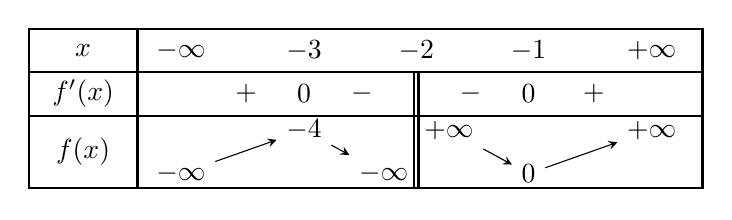
\begin{tikzpicture}[>=stealth,scale=0.92]
		  \draw[thick] (0,0) rectangle (9.3,-2.2);
		  \draw[thick] (0,-0.6) -- (9.3,-0.6);
		  \draw[thick] (0,-1.2) -- (9.3,-1.2);
		  \draw[thick] (1.5,0) -- (1.5,-2.2);
		  \draw[thick] (5.32,-0.6) -- (5.32,-2.2);
		  \draw[thick] (5.38,-0.6) -- (5.38,-2.2);
		  \node at (0.75,-0.3) {$x$};
		  \node at (0.75,-0.9) {$f'(x)$};
		  \node at (0.75,-1.7) {$f(x)$};
		  \node at (2.1,-0.3) {$-\infty$};
		  \node at (3.8,-0.3) {$-3$};
		  \node at (5.35,-0.3) {$-2$};
		  \node at (6.9,-0.3) {$-1$};
		  \node at (8.6,-0.3) {$+\infty$};
		  \node at (3.0,-0.9) {$+$};
		  \node at (3.8,-0.9) {$0$};
		  \node at (4.6,-0.9) {$-$};
		  \node at (6.1,-0.9) {$-$};
		  \node at (6.9,-0.9) {$0$};
		  \node at (7.8,-0.9) {$+$};
		  \node (p1) at (2.1,-2.0) {$-\infty$};
		  \node (p2) at (3.8,-1.4) {$-4$};
		  \node (p3) at (4.9,-2.0) {$-\infty$};
		  \node (p4) at (5.8,-1.4) {$+\infty$};
		  \node (p5) at (6.9,-2.0) {$0$};
		  \node (p6) at (8.6,-1.4) {$+\infty$};
		  \draw[->] (p1) -- (p2);
		  \draw[->] (p2) -- (p3);
		  \draw[->] (p4) -- (p5);
		  \draw[->] (p5) -- (p6);
		\end{tikzpicture}
		\end{center}
	}
	\loigiai{
		Tập xác định: $D = \mathbb{R} \setminus \{-2\}$.
		\begin{itemize}
			\item a) Ta có $y = x + \dfrac{1}{x + 2} \implies y' = \dfrac{2(x + 1)(x + 2) - (x + 1)^2}{(x + 2)^2} = \dfrac{(x + 3)(x + 1)}{(x + 2)^2}$. Do đó a) đúng.
			\item b) $y' = 0 \iff x = -3$ hoặc $x = -1$. Với $x \in (-3; -2)$ và $x \in (-2; -1)$ thì $y' < 0$, nên hàm số nghịch biến trên từng khoảng $(-3; -2)$ và $(-2; -1)$. Do đó b) đúng.
			\item c) Tại $x = -3$, hàm số đạt cực đại với giá trị cực đại $y_{\text{CĐ}} = y(-3) = \dfrac{(-3 + 1)^2}{-3 + 2} = -4 \ne 0$. Do đó c) sai.
			\item d) Bảng biến thiên đã cho thể hiện đúng các giới hạn, sự đổi dấu của đạo hàm và các giá trị cực trị. Do đó d) đúng.
		\end{itemize}
	}
\end{ex}

% Phần II Câu 2
\begin{ex}
	\macau{ID: TOAN12-BT3-0104-C14}Cho hàm số $y = f(x) = x^3 - 6x^2 + 9x - 2$. Xét tính đúng, sai của các phát biểu sau:
	\choiceTF
	{\True Tập xác định là $\mathbb{R}$}
	{Hàm số đồng biến trên khoảng $(1; 3)$}
	{\True Giá trị cực tiểu của hàm số bằng $-2$}
	{Điểm $I(2; 1)$ là tâm đối xứng của đồ thị}
	\loigiai{
		\begin{itemize}
			\item a) Hàm đa thức bậc ba có tập xác định $D = \mathbb{R}$. Do đó a) đúng.
			\item b) Ta có $f'(x) = 3x^2 - 12x + 9 = 3(x - 1)(x - 3)$. Trên khoảng $(1; 3)$, $f'(x) < 0$ nên hàm số nghịch biến trên khoảng $(1; 3)$. Do đó b) sai.
			\item c) Qua $x = 3$, $f'(x)$ đổi dấu từ âm sang dương nên hàm số đạt cực tiểu tại $x = 3$; giá trị cực tiểu $y_{\text{CT}} = f(3) = 3^3 - 6 \cdot 3^2 + 9 \cdot 3 - 2 = -2$. Do đó c) đúng.
			\item d) Điểm uốn của đồ thị hàm bậc ba là tâm đối xứng: $f''(x) = 6x - 12 = 0 \iff x = 2 \implies y = 0$. Tâm đối xứng là $I(2; 0)$, không phải $I(2; 1)$. Do đó d) sai.
		\end{itemize}
	}
\end{ex}

\newpage
% Phần II Câu 3
\begin{ex}
	\immini{\macau{ID: TOAN12-BT3-0104-C15}
		Cho hàm số phân thức $y = \dfrac{ax + b}{cx + d}$ ($ac \ne 0$, $ad - bc \ne 0$) có đồ thị như hình bên. Xét tính đúng, sai của các phát biểu sau:
		\choiceTF
		{\True Đồ thị có tiệm cận đứng $x = -2$}
		{Đồ thị có tiệm cận ngang $y = 1$}
		{\True Tâm đối xứng của đồ thị là $I(-2; -1)$}
		{Hàm số đồng biến trên từng khoảng xác định}
	}{
		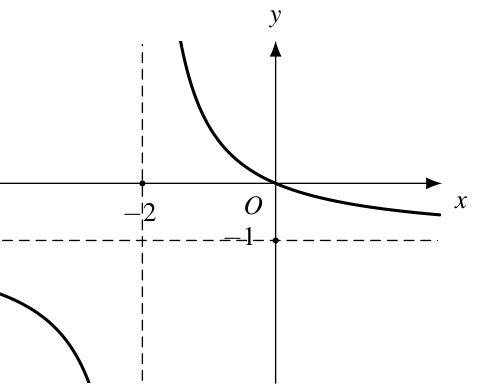
\includegraphics[width=4.0cm]{p2_c3_hinh.png}
	}
	\loigiai{
		Dựa vào đồ thị hàm số:
		\begin{itemize}
			\item a) Đường tiệm cận đứng là $x = -2$. Do đó a) đúng.
			\item b) Đường tiệm cận ngang là $y = -1$, không phải $y = 1$. Do đó b) sai.
			\item c) Giao điểm của hai đường tiệm cận là $I(-2; -1)$, đây chính là tâm đối xứng của đồ thị. Do đó c) đúng.
			\item d) Trên mỗi khoảng xác định $(-\infty; -2)$ và $(-2; +\infty)$, các nhánh đồ thị đi xuống từ trái sang phải nên hàm số nghịch biến trên từng khoảng xác định. Do đó d) sai.
		\end{itemize}
	}
\end{ex}

% Phần II Câu 4
\begin{ex}
	\immini{\macau{ID: TOAN12-BT3-0104-C16}
		Cho hàm số $y = \dfrac{-2x + 1}{x + 1}$. Xét tính đúng, sai của các phát biểu sau:
		\choiceTF
		{\True Đạo hàm là $y' = -\dfrac{3}{(x + 1)^2}$}
		{\True Hàm số nghịch biến trên từng khoảng xác định}
		{Đồ thị có tiệm cận ngang $y = 2$}
		{\True Hình bên là đồ thị của hàm số đã cho}
	}{
		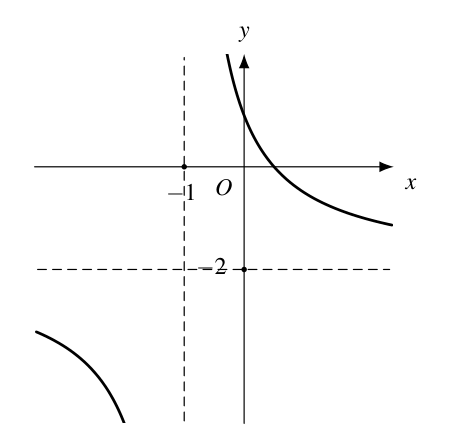
\includegraphics[width=4.0cm]{p2_c4_hinh.png}
	}
	\loigiai{
		Tập xác định: $D = \mathbb{R} \setminus \{-1\}$.
		\begin{itemize}
			\item a) Ta có $y' = \dfrac{-2(1) - 1(1)}{(x + 1)^2} = -\dfrac{3}{(x + 1)^2}$. Do đó a) đúng.
			\item b) Vì $y' < 0, \; \forall x \ne -1$ nên hàm số nghịch biến trên từng khoảng xác định $(-\infty; -1)$ và $(-1; +\infty)$. Do đó b) đúng.
			\item c) Ta có $\lim\limits_{x \to \pm\infty} y = -2$, do đó tiệm cận ngang của đồ thị là $y = -2$, không phải $y = 2$. Do đó c) sai.
			\item d) Đồ thị có tiệm cận đứng $x = -1$, tiệm cận ngang $y = -2$ và đồ thị nghịch biến trên từng khoảng xác định, hoàn toàn trùng khớp với hình vẽ. Do đó d) đúng.
		\end{itemize}
	}
\end{ex}

\newpage
\begin{flushleft}
	{\color{blue!50!green}\fbox{\fontfamily{qag}\bfseries\selectfont PHẦN III. Câu trắc nghiệm yêu cầu trả lời ngắn}}
	\textit{\small (Thí sinh trả lời từ câu 1 đến câu 6.)}
\end{flushleft}
\setcounter{ex}{0}
\setcounter{bt}{0}

% Phần III Câu 1
\begin{ex}
	\macau{ID: TOAN12-BT3-0104-C17}Cho hàm số $y = f(x) = -x^3 + 3x + 1$. Tính tổng hai giá trị cực trị của hàm số.
	\par\shortans[oly]{2}
	\loigiai{
		Ta có $f'(x) = -3x^2 + 3 = -3(x^2 - 1) = 0 \iff x = \pm 1$.\\
		Giá trị cực đại: $y_{\text{CĐ}} = f(1) = -(1)^3 + 3(1) + 1 = 3$.\\
		Giá trị cực tiểu: $y_{\text{CT}} = f(-1) = -(-1)^3 + 3(-1) + 1 = -1$.\\
		Tổng hai giá trị cực trị là: $y_{\text{CĐ}} + y_{\text{CT}} = 3 + (-1) = 2$.
	}
\end{ex}

% Phần III Câu 2
\begin{ex}
	\macau{ID: TOAN12-BT3-0104-C18}Cho hàm số $y = \dfrac{x^2 - x + 2}{x - 2}$. Gọi $I(a; b)$ là giao điểm hai đường tiệm cận của đồ thị. Tính $a + b$.
	\par\shortans[oly]{5}
	\loigiai{
		Ta thực hiện phép chia: $y = \dfrac{x^2 - x + 2}{x - 2} = x + 1 + \dfrac{4}{x - 2}$.\\
		Đường tiệm cận đứng là $x = 2$.\\
		Đường tiệm cận xiên là $y = x + 1$.\\
		Tọa độ giao điểm $I(a; b)$ là nghiệm của hệ $\begin{cases} x = 2 \\ y = x + 1 \end{cases} \implies \begin{cases} a = 2 \\ b = 3 \end{cases} \implies I(2; 3)$.\\
		Vậy $a + b = 2 + 3 = 5$.
	}
\end{ex}

% Phần III Câu 3
\begin{ex}
	\macau{ID: TOAN12-BT3-0104-C19}Cho hàm số $y = f(x)$ có đạo hàm $f'(x) = (x + 2)^2(x - 1)(x - 3)$ với mọi $x \in \mathbb{R}$. Tính tổng các giá trị của $x$ tại đó hàm số đạt cực trị.
	\par\shortans[oly]{4}
	\loigiai{
		Phương trình $f'(x) = 0 \iff x = -2$ (nghiệm kép) hoặc $x = 1$ (nghiệm đơn) hoặc $x = 3$ (nghiệm đơn).\\
		Vì $f'(x)$ chỉ đổi dấu khi qua $x = 1$ và $x = 3$ nên hàm số chỉ đạt cực trị tại hai điểm $x = 1$ và $x = 3$.\\
		Tổng các giá trị của $x$ tại đó hàm số đạt cực trị là: $1 + 3 = 4$.
	}
\end{ex}

\newpage
% Phần III Câu 4
\begin{ex}
	\macau{ID: TOAN12-BT3-0104-C20}Cho hàm số $y = \dfrac{x^2 - 2x + 5}{x - 1}$. Gọi $A, B$ là hai điểm cực trị của đồ thị hàm số. Tính độ dài đoạn thẳng $AB$ (kết quả làm tròn đến hàng phần trăm).
	\par\shortans[oly]{8,94}
	\loigiai{
		Ta có $y = x - 1 + \dfrac{4}{x - 1} \implies y' = 1 - \dfrac{4}{(x - 1)^2} = \dfrac{(x - 1)^2 - 4}{(x - 1)^2} = \dfrac{(x + 1)(x - 3)}{(x - 1)^2}$.\\
		$y' = 0 \iff x = -1$ hoặc $x = 3$.\\
		Với $x = -1 \implies y = -4 \implies A(-1; -4)$.\\
		Với $x = 3 \implies y = 4 \implies B(3; 4)$.\\
		Độ dài đoạn thẳng $AB$ là:
		\[
		AB = \sqrt{(3 - (-1))^2 + (4 - (-4))^2} = \sqrt{4^2 + 8^2} = \sqrt{80} = 4\sqrt{5} \approx 8{,}94.
		\]
	}
\end{ex}

% Phần III Câu 5
\begin{ex}
	\macau{ID: TOAN12-BT3-0104-C21}Cho hàm số $y = f(x) = \dfrac{x^2 - x + 4}{x}$. Tính hiệu giữa giá trị cực tiểu và giá trị cực đại của hàm số.
	\par\shortans[oly]{8}
	\loigiai{
		Tập xác định: $D = \mathbb{R} \setminus \{0\}$. Ta có $f(x) = x - 1 + \dfrac{4}{x} \implies f'(x) = 1 - \dfrac{4}{x^2} = \dfrac{x^2 - 4}{x^2}$.\\
		$f'(x) = 0 \iff x = \pm 2$.\\
		Hàm số đạt cực đại tại $x = -2$ với $y_{\text{CĐ}} = f(-2) = -2 - 1 + \dfrac{4}{-2} = -5$.\\
		Hàm số đạt cực tiểu tại $x = 2$ với $y_{\text{CT}} = f(2) = 2 - 1 + \dfrac{4}{2} = 3$.\\
		Hiệu giữa giá trị cực tiểu và giá trị cực đại là: $y_{\text{CT}} - y_{\text{CĐ}} = 3 - (-5) = 8$.
	}
\end{ex}

% Phần III Câu 6
\begin{ex}
	\macau{ID: TOAN12-BT3-0104-C22}Cho hàm số $y = \dfrac{ax + b}{cx + d}$ ($ac \ne 0$, $ad - bc \ne 0$) có bảng biến thiên như dưới đây:
	\begin{center}
	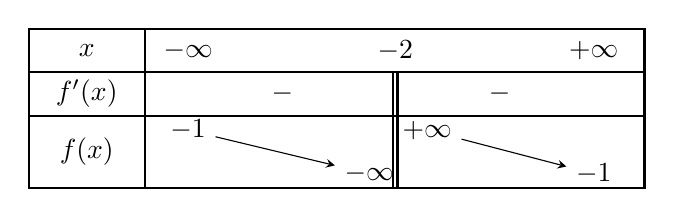
\begin{tikzpicture}[>=stealth,scale=0.92]
	  \draw[thick] (0,0) rectangle (8.5,-2.2);
	  \draw[thick] (0,-0.6) -- (8.5,-0.6);
	  \draw[thick] (0,-1.2) -- (8.5,-1.2);
	  \draw[thick] (1.6,0) -- (1.6,-2.2);
	  \draw[thick] (5.03,-0.6) -- (5.03,-2.2);
	  \draw[thick] (5.09,-0.6) -- (5.09,-2.2);
	  \node at (0.8,-0.3) {$x$};
	  \node at (0.8,-0.9) {$f'(x)$};
	  \node at (0.8,-1.7) {$f(x)$};
	  \node at (2.2,-0.3) {$-\infty$};
	  \node at (5.06,-0.3) {$-2$};
	  \node at (7.8,-0.3) {$+\infty$};
	  \node at (3.5,-0.9) {$-$};
	  \node at (6.5,-0.9) {$-$};
	  \node (p1) at (2.2,-1.4) {$-1$};
	  \node (p2) at (4.7,-2.0) {$-\infty$};
	  \node (p3) at (5.5,-1.4) {$+\infty$};
	  \node (p4) at (7.8,-2.0) {$-1$};
	  \draw[->] (p1) -- (p2);
	  \draw[->] (p3) -- (p4);
	\end{tikzpicture}
	\end{center}
	Gọi $I(u; v)$ là tâm đối xứng của đồ thị hàm số. Tính $u + v$.
	\par\shortans[oly]{-3}
	\loigiai{
		Từ bảng biến thiên của hàm số phân thức bậc nhất trên bậc nhất:
		\begin{itemize}
			\item Tiệm cận đứng là $x = -2$.
			\item Tiệm cận ngang là $y = -1$.
		\end{itemize}
		Tâm đối xứng của đồ thị là giao điểm hai tiệm cận: $I(-2; -1)$.\\
		Suy ra $u = -2, v = -1 \implies u + v = -2 + (-1) = -3$.
	}
\end{ex}
